\documentclass[11pt,a4paper]{article}
\usepackage[T1]{fontenc}
\usepackage[utf8]{inputenc}
\usepackage{amsmath,amssymb}
\usepackage{booktabs}
\usepackage{graphicx}
\usepackage[margin=2.5cm]{geometry}
\usepackage{hyperref}
\usepackage{array}

\newcommand{\kBT}{k_BT}
\newcommand{\dd}{\mathrm{d}}
\newcommand{\umps}{\,\mu\mathrm{m\,s^{-1}}}
\newcommand{\tauz}{\tau_{c,0}}

\title{Soft-device closure for the $h$-model of actin--myosin interaction:\\
definitions, imposed quantities, protocols and results}
\author{}
\date{14 October 2026}

\begin{document}
\maketitle

\begin{abstract}
\noindent
We implement the $h$-model of Chaintron, Caruel and Kimmig (Math.\ in Action 12, 2023) with $N$ heads, and we add a closure for the sliding variable $x_c$ in which the \emph{total force} is imposed and the sliding speed is an output (soft device). This note states what is imposed and what is measured in each numerical experiment, defines every plotted quantity, and reports the results, including the S-shaped force--speed relation that appears when lengthening speeds are allowed. Calibration choices that are inferred rather than read from the paper are listed explicitly in Section~\ref{sec:caveats}.
\end{abstract}

\section{Setting}

The paper computes the force--velocity curve in \emph{velocity clamp}: the sliding velocity $\dot x_c$ is imposed and the mean force per head $\tau_c$ is measured (its Fig.~5.2). In a force experiment the roles are reversed. Here we do both, with the same head-level model, and relate them:
\begin{itemize}
\item velocity clamp gives the curve $\tau_{ss}(u)$, with $u=-\dot x_c$;
\item the soft device imposes a load, adds a macroscopic viscosity $\nu$ on $x_c$, and measures $u(t)$.
\end{itemize}
The two are linked by a steady-state relation (Section~\ref{sec:steady}) whose non-monotone part produces the S.

\section{The \texorpdfstring{$h$}{h}-model as implemented}

\subsection{State, units, geometry}
Head $i=1,\dots,N$ carries $(\alpha_i,X_i,h_i)$: $\alpha_i\in\{0,1\}$ (detached/attached), $X_i$ the position of the tip relative to its anchor, and $h_i\in[-d/2,d/2)$ the signed distance from the tip to the nearest actin site, so that the site is at $X_i+h_i$. When attached, $X_i$ is the site position and $h_i=0$. Units are nm, ms, pN, zJ ($1\,\mathrm{pN\,nm}=1\,\mathrm{zJ}$); $\mu\mathrm m/\mathrm s\equiv\mathrm{nm/ms}$. We use $d=40$ nm, $T=298$ K, $\kBT\simeq 4.11$ zJ, $\mu_T=100$ zJ, and the micro drag $\eta=0.097$ pN\,ms/nm of the detached tip.

\subsection{Energies and force per head}
The detached and attached energies $w_0,w_1$ are the regularised piecewise quadratic potentials of Table~D.1 (Appendix~\ref{app:params}). A head transmits to the actin only when attached:
\begin{equation}
f_i=\alpha_i\,w_1'(X_i).
\end{equation}
The paper's $\tau_c(t)=\int\partial_xw_1\,p(t,1,x)\,\dd x$ is the expectation of one $f_i$; we estimate it by $\hat\tau(t)=N^{-1}\sum_i f_i$. The attached fraction is $n_a=N^{-1}\sum_i\alpha_i$ and the force per attached head is $\check\tau_c=\tau_c/n_a$.

\subsection{Jumps and detailed balance}
There are four channels, each with its own clock $c$ and threshold $e\sim\mathcal E(1)$ (Algorithm~1 of the paper):
\begin{center}
\begin{tabular}{cll}
\toprule
channel & transition & rate \\
\midrule
A & $0\to1$ (direct attachment) & $K_{0\to1}(x,h)$ \\
B & $0\to1$ (reverse of detachment) & $K^{\rm rev}_{1\to0}(x,h)$ \\
C & $1\to0$ (direct detachment) & $k_{1\to0}(x)=\int K_{1\to0}(x,h)\,\dd h$ \\
D & $1\to0$ (reverse of attachment) & $k^{\rm rev}_{0\to1}(x)=\int K^{\rm rev}_{0\to1}(x,h)\,\dd h$ \\
\bottomrule
\end{tabular}
\end{center}
$K_{0\to1}$ and $K^{\rm rev}_{1\to0}$ are the primitive rates of Table~D.1. The other two follow from detailed balance. With the pairing $x_{\rm det}=x_{\rm att}-h$,
\begin{align}
K^{\rm rev}_{0\to1}(x_{\rm att},h)&=\frac1d\,K_{0\to1}(x_{\rm att}-h,h)\,\exp\!\Big[\frac{w_1(x_{\rm att})-w_0(x_{\rm att}-h)}{\kBT}\Big],\\
K_{1\to0}(x_{\rm att},h)&=\frac1d\,K^{\rm rev}_{1\to0}(x_{\rm att}-h,h)\,\exp\!\Big[\frac{w_1(x_{\rm att})-w_0(x_{\rm att}-h)+\mu_T}{\kBT}\Big].
\end{align}
The factor $1/d$ is discussed in Section~\ref{sec:caveats}. On detachment through C or D, the landing value $h'$ is drawn from the corresponding density $K_{1\to0}(x_{\rm att},\cdot)$ or $K^{\rm rev}_{0\to1}(x_{\rm att},\cdot)$, using tabulated cumulative distributions.

\subsection{Time stepping}
At each step $\delta t=0.002$ ms: (i) compute $\sum_i f_i$ and fix $\Delta x_c$ (Section~\ref{sec:closure}); (ii) update the clocks of the active channels (A, B if detached; C, D if attached) and select the channel with the largest positive residual $c-e$, if any; (iii) move detached tips by Euler--Maruyama, $\Delta X=-\eta^{-1}w_0'(X)\delta t+\sqrt{2\kBT\delta t/\eta}\,\xi$, with $h\leftarrow h+\Delta x_c-\Delta X \pmod d$, and move attached tips by $\Delta x_c$; (iv) apply jumps: attachment sets $X\leftarrow X+h+\Delta x_c$, $h\leftarrow0$; detachment sets $X\leftarrow X+\Delta x_c-h'$, $h\leftarrow h'$; (v) reset the clocks of jumping heads.

\section{Imposing the sliding}
\label{sec:closure}

\subsection{Conventions}
Following the paper, $\dot x_c<0$ is contraction and $f_i>0$ is traction. We use the shortening speed $u=-\dot x_c$ (so $u<0$ is lengthening). All $x_c$-dependence of the energy is through the attached heads, $E=\sum_i\alpha_iw_1(X_i)$ with $\partial X_i/\partial x_c=1$ for an attached head, hence $\partial E/\partial x_c=\sum_if_i$.

\subsection{Velocity clamp (the paper's protocol)}
$\dot x_c=v$ is prescribed. Heads are then independent, and an ensemble of $N$ heads with random initial $h_i$ is simply a Monte Carlo sample of one head. We measure the time averages $\langle\hat\tau\rangle$ and $\langle n_a\rangle$ after a burn-in. Defining
\begin{equation}
\tau_{ss}(u):=\langle\hat\tau\rangle\big|_{\dot x_c=-u}
\end{equation}
gives the force--velocity curve of Fig.~5.2, now also for $u<0$.

\subsection{Soft device}
The actin is rigid with coordinate $x_c$, subject to a viscous drag $\nu\dot x_c$, an external force and the motor force. Overdamped balance gives
\begin{equation}
\nu\,\dot x_c=-F_{\rm ext}-\sum_{i=1}^N f_i,
\qquad\text{i.e.}\qquad
F_{\rm ext}+\sum_i f_i+\nu\dot x_c=0 .
\label{eq:closure}
\end{equation}
$F_{\rm ext}>0$ assists contraction; a load opposing contraction is $P=-F_{\rm ext}$. At $\dot x_c=0$ it reduces to $F_{\rm ext}+\sum_if_i=0$. This is the same update as the $\delta s$ step of the earlier $N$-head JAP codes, with $v\leftrightarrow\nu$ and $F\leftrightarrow-F_{\rm ext}$.

\paragraph{Per-head form.} With $\tilde\nu=\nu/N$ and $\bar p=P/N=-F_{\rm ext}/N$,
\begin{equation}
\tilde\nu\,\dot x_c=\bar p-\hat\tau
\quad\Longleftrightarrow\quad
\hat\tau=\bar p+\tilde\nu\,u .
\label{eq:perhead}
\end{equation}
Since the force on the filament is $N\tau_c$ and not $\tau_c$, the sum in \eqref{eq:closure} is $N\hat\tau$.

\paragraph{Numerics.} At fixed $\alpha$, $\frac{\dd}{\dd t}\sum f=K\dot x_c$ with $K=\sum_i\alpha_i\max(w_1''(X_i),0)$, which makes \eqref{eq:closure} stiff with rate $K/\nu$. We use the semi-implicit step
\begin{equation}
\Delta x_c=-\frac{(F_{\rm ext}+\sum_if_i)\,\delta t}{\nu+K\,\delta t}.
\end{equation}
There is no thermal noise on $x_c$.

\subsection{What is imposed and what is measured}
\begin{center}
\begin{tabular}{p{3.3cm}p{5.2cm}p{5.5cm}}
\toprule
experiment & imposed & measured \\
\midrule
isometric & $\dot x_c=0$ & $\langle n_a\rangle$, $\langle\hat\tau\rangle$, $\check\tau_c$ \\
velocity-clamp sweep & $\dot x_c=v$, 21 values from $+6$ to $-15\umps$ & $\langle\hat\tau\rangle$, $\langle n_a\rangle$ $\Rightarrow\tau_{ss}(u)$ \\
soft-device ramp & $F_{\rm ext}(t)=-N\bar p(t)$, $\nu=N\tilde\nu$ & $x_c(t)$, hence $u(t)$; also $\hat\tau$, $n_a$ \\
\bottomrule
\end{tabular}
\end{center}
Common settings. Velocity clamp: $N=400$, $T=60$ ms, burn-in 15 ms, $\delta t=0.002$ ms. Soft ramp: $\bar p(t)$ is piecewise linear, held at $0.22$ pN for 60 ms, raised to $1.144$ pN over 300 ms, and lowered back over 300 ms ($0.245\to1.272$ in units of $\tauz=0.899$ pN); $\tilde\nu\in\{0.05,0.30\}$ pN\,ms/nm and $N\in\{30,100,300\}$. All runs start with every head detached, $h$ uniform on $[-d/2,d/2)$, and the tip drawn from a Gaussian around $x=-2$ nm.

\section{Steady states under force control and the S}
\label{sec:steady}

\subsection{Steady-state relation}
In a steady state at speed $u$ the mean force is $\tau_{ss}(u)$, so \eqref{eq:perhead} gives the load that sustains that speed:
\begin{equation}
\bar p(u)=\tau_{ss}(u)-\tilde\nu\,u .
\label{eq:pbar}
\end{equation}
For $\tilde\nu\to0$ this is the paper's curve, which is the experimental force-clamp protocol. A positive $\tilde\nu$ shifts each point horizontally by $-\tilde\nu u$.

\subsection{Stability (heuristic)}
Assume the head population relaxes to $\tau_{ss}$ with a single time $\theta$, $\theta\dot\tau=\tau_{ss}(u)-\tau$, with $u=(\tau-\bar p)/\tilde\nu$ from \eqref{eq:perhead}. Linearising,
\begin{equation}
\theta\,\delta\dot\tau=\Big(\frac{\tau_{ss}'(u)}{\tilde\nu}-1\Big)\delta\tau,
\end{equation}
so a steady state is stable if and only if $\tau_{ss}'(u)<\tilde\nu$, equivalently $\dd\bar p/\dd u<0$. This is a one-timescale argument; the real population relaxes on several timescales, so it should be read as a criterion for the sign, not for the location.

\subsection{Origin of the fold}
Where $\tau_{ss}$ is non-monotone, $\bar p(u)$ is multivalued as a function of the load. We measured $\tau_{ss}$ decreasing monotonically for lengthening ($u<0$), and a slight rise for small $u>0$ (from $0.88$ to $0.94$ pN, comparable to the scatter), as the paper also notes for small shortening speeds. For $\tilde\nu=0.05$ this leaves a stable shortening branch ending at $\bar p\simeq1.03\,\tauz$ ($u\simeq0.2$), an unstable stretch around the stall point, and a fast-lengthening branch $u\simeq(\bar p-\hat\tau)/\tilde\nu$ whose minimum load is $\simeq0.59\,\tauz$ at $|u|\simeq3$. Increasing $\tilde\nu$ removes the fold (Table~\ref{tab:fold}).

\begin{table}[h]
\centering
\begin{tabular}{ccc}
\toprule
$\tilde\nu$ (pN\,ms/nm) & max of $\bar p$ on stall/shortening side & min of $\bar p$ on lengthening side \\
\midrule
0.05 & $1.03\,\tauz$ at $u=0.2$ & $0.59\,\tauz$ at $u=-3$ \\
0.15 & $1.02\,\tauz$ & $0.85\,\tauz$ at $u=-1.5$ \\
0.30 & $1.07\,\tauz$ & $0.98\,\tauz$ at $u=-0.7$ \\
\bottomrule
\end{tabular}
\caption{Fold positions obtained from \eqref{eq:pbar} with the measured $\tau_{ss}$ (linear interpolation, $\tauz=0.899$ pN). For $\tilde\nu=0.30$ the fold depth, $0.09\,\tauz$, is of the order of the scatter of $\tau_{ss}$.}
\label{tab:fold}
\end{table}

\section{What the figure shows}

\begin{figure}[h]
\centering
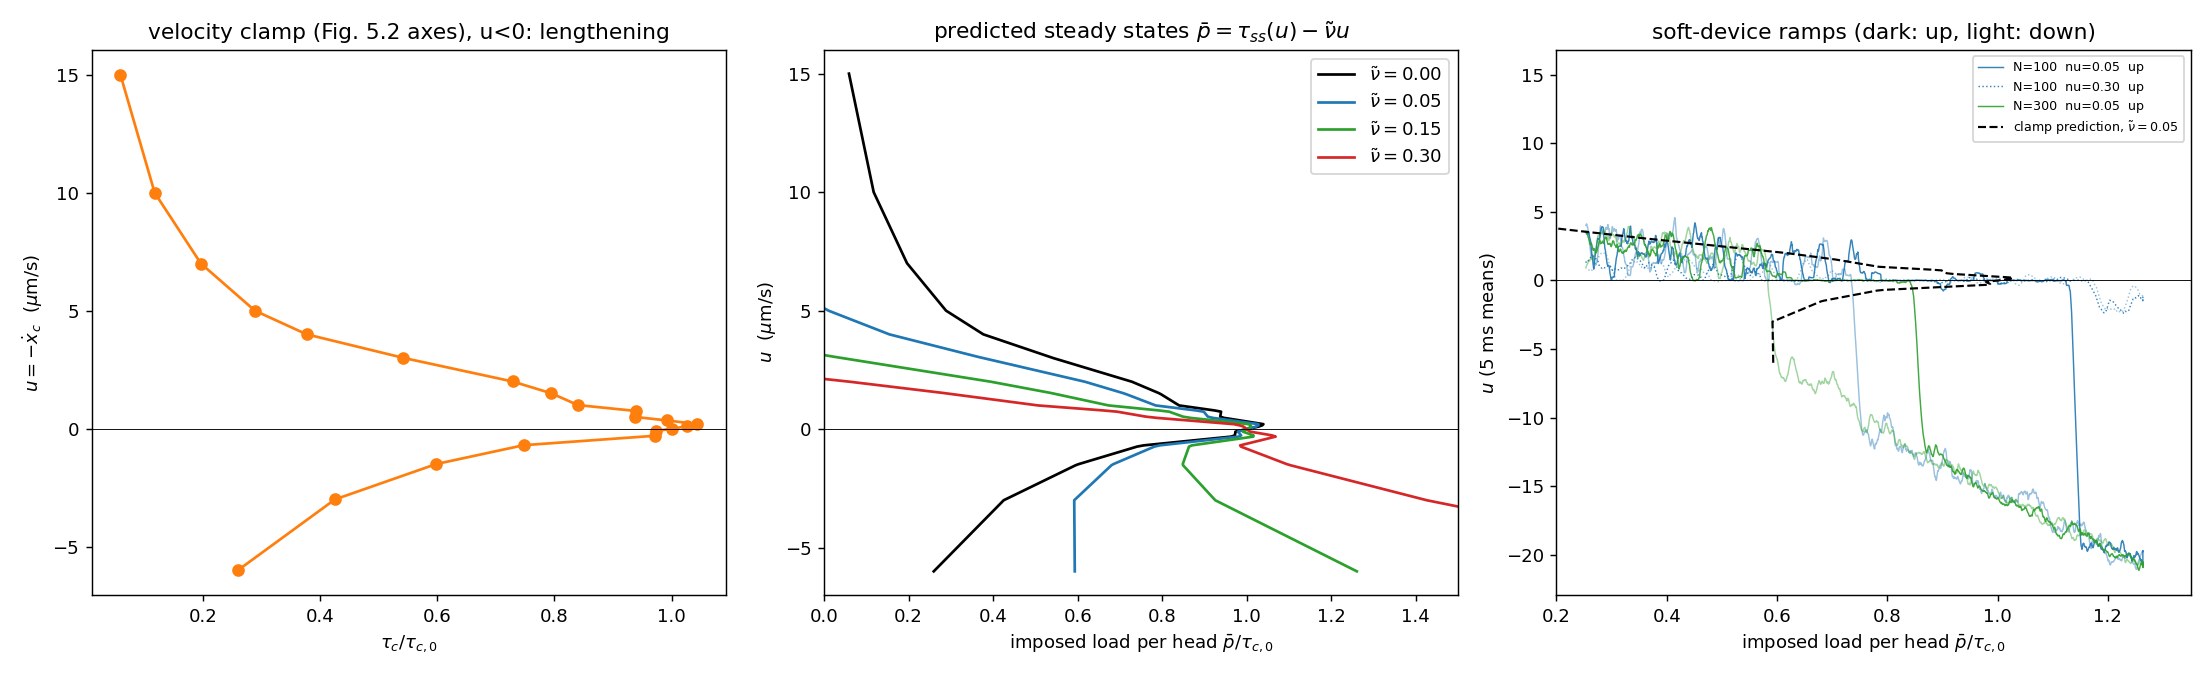
\includegraphics[width=\textwidth]{S_curve.png}
\caption{Left: velocity-clamp curve. Middle: steady-state load from \eqref{eq:pbar}. Right: soft-device ramps.}
\label{fig:S}
\end{figure}

\paragraph{Left panel (simulation, velocity clamp).} Horizontal axis: $\langle\hat\tau\rangle/\tauz$, mean force per head. Vertical axis: $u=-\dot x_c$ in $\mu$m/s; $u>0$ is shortening and $u<0$ is lengthening. Each marker is one clamp run of $N=400$ heads with $\dot x_c$ imposed. The point at $u=0$ is replaced by the mean of $u=\pm0.1$ because at $\dot x_c=0$ the ensemble is quenched in $h$ and its mean depends on the sample. $\tauz$ is the value at $u\approx0$, $0.899$ pN.

\paragraph{Middle panel (no new simulation).} It is the transformation \eqref{eq:pbar} applied to the left-panel data, with the horizontal axis now the imposed load per head $\bar p/\tauz$. Each line is one value of $\tilde\nu$; the black line is $\tilde\nu=0$ and equals the left panel. The axes are cut to $0\le\bar p/\tauz\le1.5$.

\paragraph{Right panel (simulation, soft device).} Horizontal axis: the imposed load $\bar p(t)/\tauz$ at the midpoint of a window. Vertical axis: $u=-[x_c(t+5\,\mathrm{ms})-x_c(t)]/5\,\mathrm{ms}$, the speed averaged over 5 ms. Dark lines are the upward ramp, light lines the downward ramp; solid is $\tilde\nu=0.05$ (colours: $N=30,100,300$), dotted is $\tilde\nu=0.30$ with $N=100$. The dashed black line is the middle-panel prediction for $\tilde\nu=0.05$. Here the load is the input and $u$ is an output, so jumps appear as vertical segments.

\section{Results}

\subsection{Validation}
\begin{itemize}
\item \emph{Thermodynamic consistency.} At $\mu_T=0$ with $\dot x_c=0$ the net cycling vanishes: $(A-D)/(A+D)=0.002$ and $(C-B)/(C+B)=-0.003$ ($N=600$, 90 ms). At $\mu_T=100$ zJ the net flux is positive.
\item \emph{Isometric indicators} (Table~5.1: $n_a=0.151$, $\check\tau_c=6.39$ pN). We obtain $n_a\simeq0.14$--$0.15$ and $\check\tau_c\simeq5$--$6$ pN, depending on the seed. The spread reflects the quenched $h$ distribution.
\item \emph{Force--velocity curve (Fig.~5.2).} $\tau/\tauz\simeq0.29$ at $u=5\umps$ and $\simeq0.06$ at $15\umps$, which agrees with the curve as read from the figure.
\item \emph{Closure.} In the soft-device runs $\bar p+\tilde\nu u=\hat\tau$ holds to within 0.003 pN in 40 ms windows.
\end{itemize}

\subsection{Velocity-clamp data}
\begin{table}[h]
\centering
\begin{tabular}{rcc@{\qquad}rcc}
\toprule
$u$ & $\langle\hat\tau\rangle$ (pN) & $\langle n_a\rangle$ & $u$ & $\langle\hat\tau\rangle$ (pN) & $\langle n_a\rangle$ \\
\midrule
$-6$   & 0.233 & 0.034 & $0.35$ & 0.892 & 0.145 \\
$-3$   & 0.382 & 0.056 & $0.5$  & 0.843 & 0.134 \\
$-1.5$ & 0.538 & 0.082 & $0.75$ & 0.845 & 0.139 \\
$-0.7$ & 0.672 & 0.106 & $1$    & 0.756 & 0.129 \\
$-0.3$ & 0.874 & 0.140 & $1.5$  & 0.715 & 0.138 \\
$-0.1$ & 0.875 & 0.142 & $2$    & 0.655 & 0.140 \\
$0$ (quenched) & 0.661 & 0.121 & $3$ & 0.488 & 0.133 \\
$0.1$  & 0.923 & 0.148 & $4$    & 0.339 & 0.129 \\
$0.2$  & 0.938 & 0.154 & $5$    & 0.260 & 0.117 \\
       &       &       & $7$    & 0.177 & 0.092 \\
       &       &       & $10$   & 0.106 & 0.079 \\
       &       &       & $15$   & 0.053 & 0.059 \\
\bottomrule
\end{tabular}
\caption{Velocity clamp, $N=400$, one run per speed. Errors were not estimated by repetition; the scatter between neighbouring speeds (for example $u=-0.3$ and $-0.7$) suggests $\pm0.05$--$0.1$ pN.}
\end{table}

\subsection{Soft-device ramps}
\begin{table}[h]
\centering
\begin{tabular}{ccccp{5.2cm}}
\toprule
$N$ & $\tilde\nu$ & yield load & recapture load & remark \\
\midrule
30  & 0.05 & $1.15\,\tauz$ & intermittent & rescues up to $1.23\,\tauz$, no clean loop \\
100 & 0.05 & $1.14\,\tauz$ & $0.74\,\tauz$ & hysteresis loop \\
300 & 0.05 & $0.85\,\tauz$ & $0.59\,\tauz$ & recapture at predicted floor \\
100 & 0.30 & none & none & max lengthening speed $2.4\umps$, reversible \\
\bottomrule
\end{tabular}
\caption{Yield: first upward-ramp time with the 5 ms mean $u<-3\umps$. Recapture: first downward-ramp time after the filament has been below $-10\umps$ at which $u>-3\umps$. One realisation per row; $\tauz=0.899$ pN. Predicted for $\tilde\nu=0.05$, $N\to\infty$: yield $1.03\,\tauz$, floor $0.59\,\tauz$.}
\end{table}

The upward ramp follows the shortening branch, stalls ($u\approx0$) close to $\tauz$, and then yields to lengthening at speeds up to $\simeq21\umps$ ($\simeq(\bar p-\hat\tau)/\tilde\nu$, with few heads attached). On the way down the filament stays on the fast branch until a load that depends on $N$. For $\tilde\nu=0.30$ there is no runaway.

\subsection{Dependence on \texorpdfstring{$N$}{N}}
Equation \eqref{eq:pbar} is the $N\to\infty$ limit. At finite $N$, $u=(\hat\tau-\bar p)/\tilde\nu$ inherits the fluctuations of $\hat\tau$, of order $\sigma_f/\sqrt N$ with $\sigma_f$ the standard deviation of one $f_i$ (a Bernoulli estimate gives $\sigma_f\approx\sqrt{n_a(1-n_a)}\,\check\tau_c\approx2$ pN). The fluctuation of the speed is then $\delta u\sim\sigma_f/(\tilde\nu\sqrt N)$, about $4\umps$ for $N=100$ and $\tilde\nu=0.05$ (an order-of-magnitude estimate), comparable to the mean speed. This is consistent with what we observe: at $N=100$, $\tilde\nu=0.05$ and $\bar p=0.28$ pN the mean speed is $2.45\umps$ with $\hat\tau=0.41$ pN and $n_a=0.14$, whereas the clamp curve gives $\tau_{ss}(2.45)\simeq0.58$ pN at the same $n_a$. The mean force per attached head is lower in the soft device because heads experience a fluctuating speed.

Two trends are supported by the data: the recapture load moves toward the predicted floor as $N$ grows ($0.74\to0.59$), and the $N=30$ system does not stay on either branch. The yield loads ($1.15,1.14,0.85$) are not monotone in $N$ and come from single runs, so no trend is claimed for them.

\section{Caveats and limitations}
\label{sec:caveats}
\begin{enumerate}
\item \textbf{Factor $1/d$ in the detailed-balance rates.} Taken literally, (3.4)--(3.5) of the paper give $n_a=0.03$. Since $K_{0\to1}$ and $K^{\rm rev}_{1\to0}$ are rates while $K_{1\to0}$ and $K^{\rm rev}_{0\to1}$ are densities in $h$, the relation needs a length, and for the uniform measure on the torus it is $d$ (parameter \texttt{H\_NORM}). With it, $n_a$ matches Table~5.1. The $\mu_T=0$ test passes for any value of this factor, so it does not validate it.
\item \textbf{Potentials.} Evaluated from Table~D.1 as extracted from the PDF text, $w_1$ and $w_0$ agree with Fig.~5.1(a) in the difference $w_0-w_1$ at the minima ($\approx77$ zJ) but differ by a constant of about 30 zJ in absolute value. A constant cancels in all rates. I did not compare the curves point by point.
\item \textbf{Table D.1 reading.} The box in $x$ of $K_{0\to1}$ is taken as $[x^+_\ell,x^+_r]=[1.5,17]$ nm (a positive interval, as in the text of Section~5.1); the exponent in $K^{\rm rev}_{1\to0}$ is clipped to $\pm30$ for numerical safety. The paper's text and Table~D.1 are not fully consistent about which of $K_{1\to0}$, $K^{\rm rev}_{1\to0}$ is the primitive rate; I took the table at face value.
\item \textbf{Statistics.} One run per velocity and per $(N,\tilde\nu)$ in the ramps; no repeated runs, no confidence intervals, and no time-step convergence study (all runs use $\delta t=0.002$ ms).
\item \textbf{Free parameter.} $\tilde\nu$ is not given by the paper; $0.05$ and $0.30$ are my choices.
\item \textbf{No noise on $x_c$.} The closure is deterministic, so at finite $N$ and $\mu_T=0$ the stationary law is not the soft-ensemble Gibbs measure.
\item \textbf{Heuristics.} The stability criterion of Section~\ref{sec:steady} assumes one relaxation time, and the $\delta u$ estimate is of order of magnitude only.
\item \textbf{Range.} The clamp sweep reaches $u=-6\umps$ on the lengthening side, whereas the ramps explore lengthening up to $-21\umps$.
\end{enumerate}

\section{Reproducing}
\begin{center}
\begin{tabular}{ll}
\toprule
file & role \\
\midrule
\texttt{hmodel\_soft.py} & engine: potentials, rates, tables, \texttt{run(...)} with modes \texttt{clamp} and \texttt{soft} \\
\texttt{sweep\_clamp.py} & velocity-clamp sweep, writes \texttt{clamp\_sweep.npy} \\
\texttt{soft\_ramp.py N nu} & force ramp up and down, writes \texttt{ramp\_*.npz} \\
\texttt{plot\_S.py} & builds Fig.~\ref{fig:S} from the two outputs \\
\bottomrule
\end{tabular}
\end{center}
In \texttt{soft\_ramp.py} the reference force is hard-coded as $0.88$ pN to define the ramp limits; the measured $\tauz$ is $0.899$ pN, and all normalised results here use the latter.

\appendix
\section{Parameters}
\label{app:params}
\begin{center}
\begin{tabular}{ll}
\toprule
quantity & value \\
\midrule
$w_1$ ($\kappa_\ell,\kappa_r,\tilde x_\ell,\tilde x_r,x_\alpha,x_\ell,x_r,\check w,E$) & $0.60,\ 1,\ -12.5,\ -1.5,\ 2,\ 1.3,\ 2.5,\ 5.7,\ 50$ \\
$w_0$ (same order) & $0.12,\ 1,\ -2,\ 2,\ -2,\ -3.5,\ 0.5,\ 5.7,\ 70$ \\
$K_{0\to1}$: $k_{\max}^+,\lambda_h^+,h_{1/2}^+,\lambda_x^+,x_\ell^+,x_r^+$ & $0.413,\ 1.6,\ 3.9,\ 8,\ 1.5,\ 17$ \\
$K^{\rm rev}_{1\to0}$: $k_{\max},\lambda_h,h_{1/2},\lambda_x,x$ (first term) & $0.206,\ 5,\ 2,\ 10,\ -28$ \\
\quad second term: $k_p,\lambda_h,h_{1/2},\lambda_x,x_p$ & $3.1,\ 5,\ 2,\ 20,\ 0.5$ \\
\quad third term: $k_b,\lambda_h,h_{1/2}$ & $0.07,\ 5,\ 0.2$ \\
\bottomrule
\end{tabular}
\end{center}
Units: stiffnesses in pN/nm, lengths in nm, energies in zJ, rates in ms$^{-1}$.

\section{Rate formulas}
Let $b(h;\lambda,a)=\tfrac12[1+\tanh\lambda(h+a)]$ for $h<0$ and $\tfrac12[1-\tanh\lambda(h-a)]$ for $h\ge0$. Then
\begin{align}
K_{0\to1}(x,h)&=k_{\max}^+\,b(h;\lambda_h^+,h_{1/2}^+)\,\chi(x),\\
\chi(x)&=\begin{cases}\tfrac12[1+\tanh\lambda_x^+(x-x_\ell^+)],&x<\tfrac12(x_\ell^++x_r^+),\\[2pt]\tfrac12[1-\tanh\lambda_x^+(x-x_r^+)],&\text{otherwise,}\end{cases}\\
K^{\rm rev}_{1\to0}(x,h)&=k_{\max}\,\tfrac12[1-\tanh\lambda_x(x-x_{\rm m})]\,b(h;\lambda_h,h_{1/2})\nonumber\\
&\quad+\Big\{k_p\,\tfrac12[1-\tanh\lambda_{x,p}(x-x_p)]\,b(h;5,2)+k_b\,b(h;5,0.2)\Big\}\,e^{[w_0(x)-w_1(x+h)-\mu_T]/\kBT}.
\end{align}

\end{document}
